
\setbeamerfont{block title}{size=\scriptsize}
\setbeamerfont{block body}{size=\scriptsize}
\setbeamerfont{exampleblock title}{size=\scriptsize}
\setbeamerfont{exampleblock body}{size=\scriptsize}

\begin{frame}{Les systèmes de systèmes}
% \begin{columns}[t]
%  \begin{column}{5cm}
%\begin{figure}
%\centering
%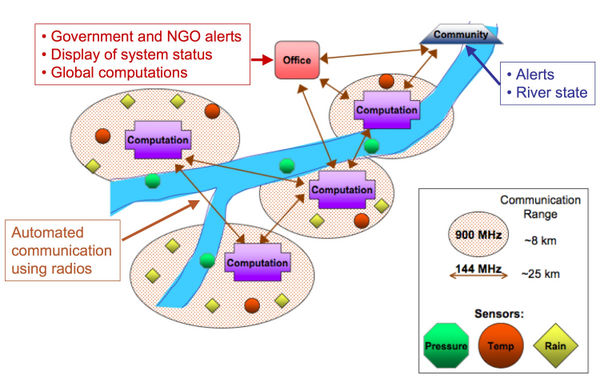
\includegraphics[width=0.5\textwidth]{imgs/fms.jpeg}\\
%Surveillance d'inondation
%\end{figure}
%\begin{figure}
%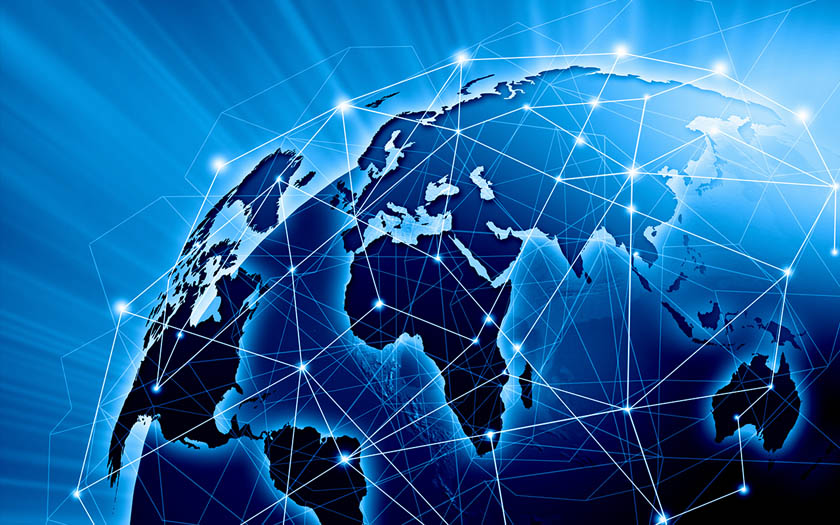
\includegraphics[width=0.5\textwidth]{imgs/internet.jpg}\\
%Internet
%\end{figure}
% \end{column}
%\begin{column}{5cm}
%\begin{figure}
%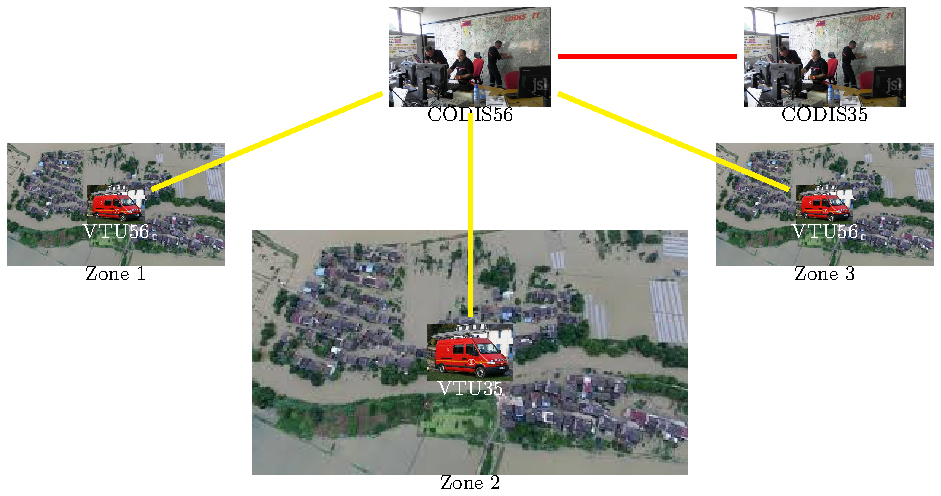
\includegraphics[width=0.5\textwidth]{imgs/fig_overview_conf1.pdf}\\
%Services d'urgence
%\end{figure}
%\begin{figure}
%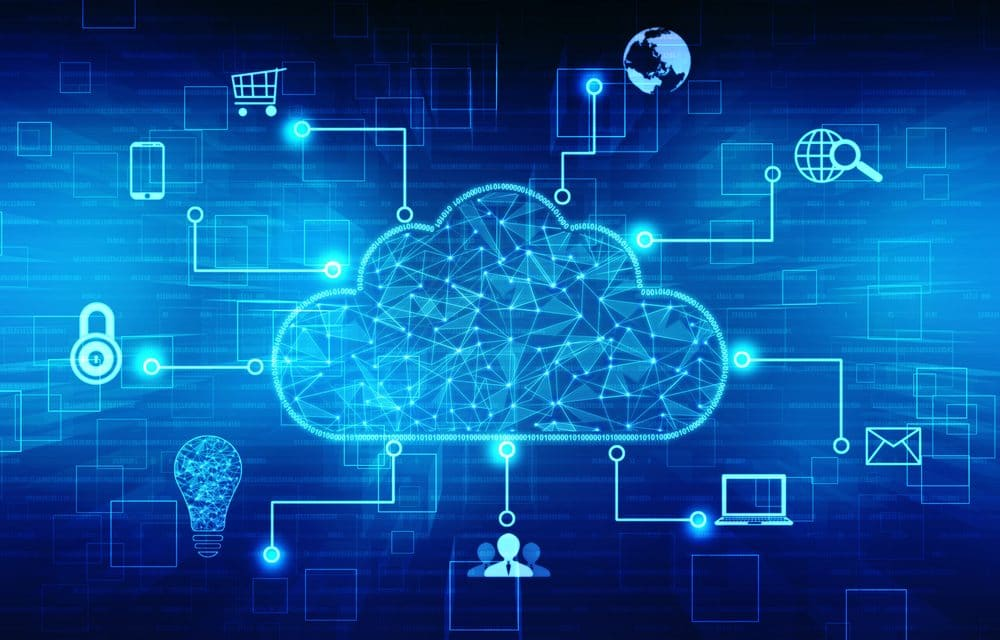
\includegraphics[width=0.5\textwidth]{imgs/web.jpg}\\
%Web
%\end{figure}
% \end{column}
% \end{columns} 
\centering 
\begin{tabular}{cc}
Dirigé & Consensuel \\
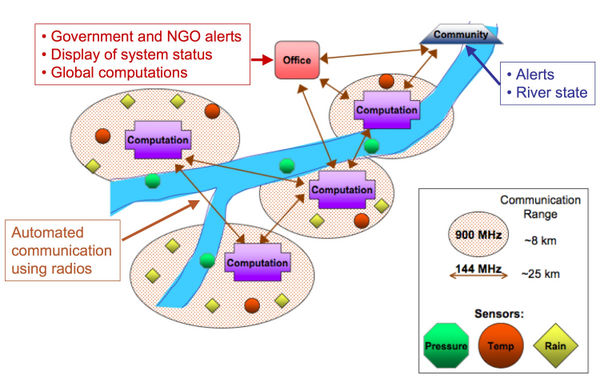
\includegraphics[width=3cm, height=2cm]{imgs/fms.jpeg} &
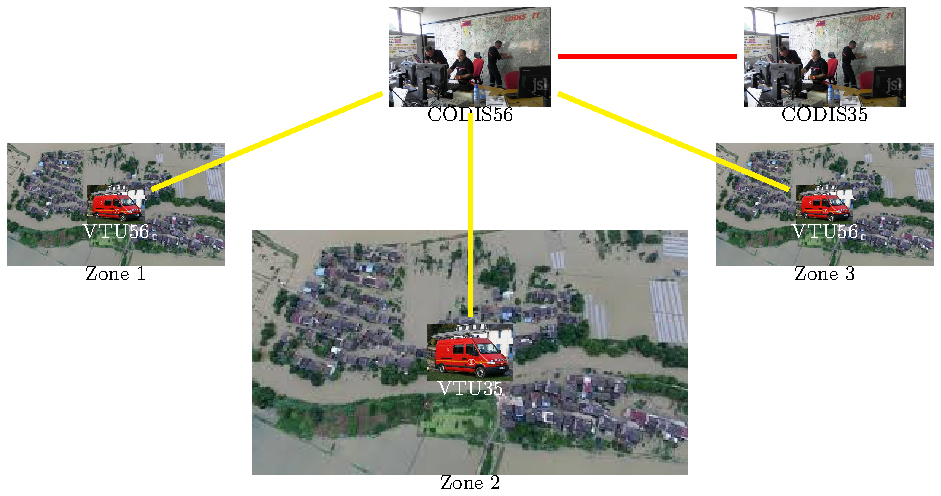
\includegraphics[width=3cm, height=2cm]{imgs/fig_overview_conf1.pdf}\\
Surveillance d'inondation \vspace{0.2cm}& Service d'urgence\vspace{0.2cm}\\
Collaboratif & Virtuel \\ 
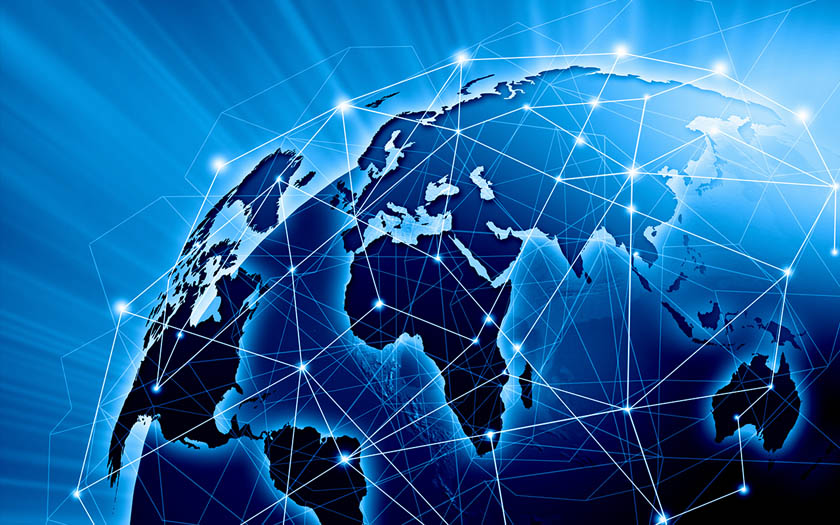
\includegraphics[width=3cm, height=2cm]{imgs/internet.jpg} &
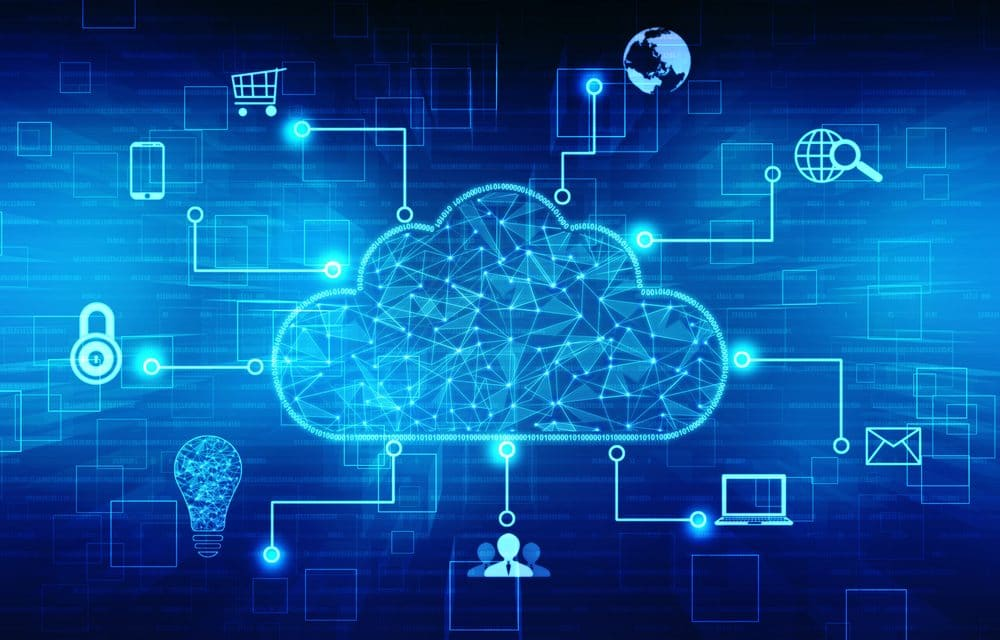
\includegraphics[width=3cm, height=2cm]{imgs/web.jpg}\\
Internet & Web \\
\end{tabular}
\begin{definition}
 Les SdSs sont des systèmes dont les composants sont géographiquement
distribués, possèdent leur propre indépendance opérationnelle et
managériale. 
L'intéraction de ces composants produit un comportement émérgent. Le
SdS a un développement évolutionnaire. 
\end{definition}
\end{frame}

\begin{frame}{Développement évolutionnaire}
\begin{definition}{}
Le \textbf{développement évolutionnaire} est l'évolution constante des
fonctions et buts du SdS. Les fonctions et les buts du SdS changent
dynamiquement et de nouveaux constituants peuvent être assemblés pour
les réaliser.
\end{definition}

\begin{columns}[t]
\begin{column}{5cm}
Raisons : 
\begin{itemize}
\item environnement opérationnel pas maîtrisé
\item indépendance managériale
\item etc.
\end{itemize}
\end{column}
\begin{column}{5cm}
\begin{figure}
\centering

\includegraphics[scale=0.4]{imgs/evolutionnaire.png}
\end{figure}
\end{column}
\end{columns}
\end{frame}

%\begin{frame}{Pré-pondérance du logiciel dans la conception SdS \& impacte du développement évolutionnaire sur les artefacts logiciels}
%\centering
%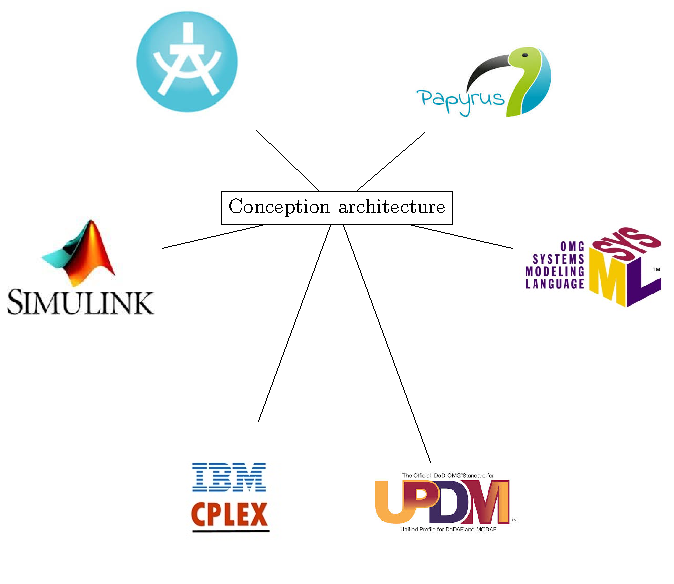
\includegraphics[scale=0.7]{imgs/logiciel.pdf}
%\end{frame}


\begin{frame}{Problématique abordée : reconfiguration dynamique}
\begin{definition}
La \textbf{reconfiguration dynamique} est une phase du
developpement d'une système qui consiste à le modifier pendant qu’il est
utilisé. La reconfiguration peut-être corrective, fonctionnelle,  ou
non-fonctionnelle.
\end{definition}
\begin{figure}
inclure schéma? 
\end{figure}
\end{frame}

\begin{frame}{Objectif : appliquer principe des patrons de conception logiciels à la reconfiguration dynamique}
\begin{figure}
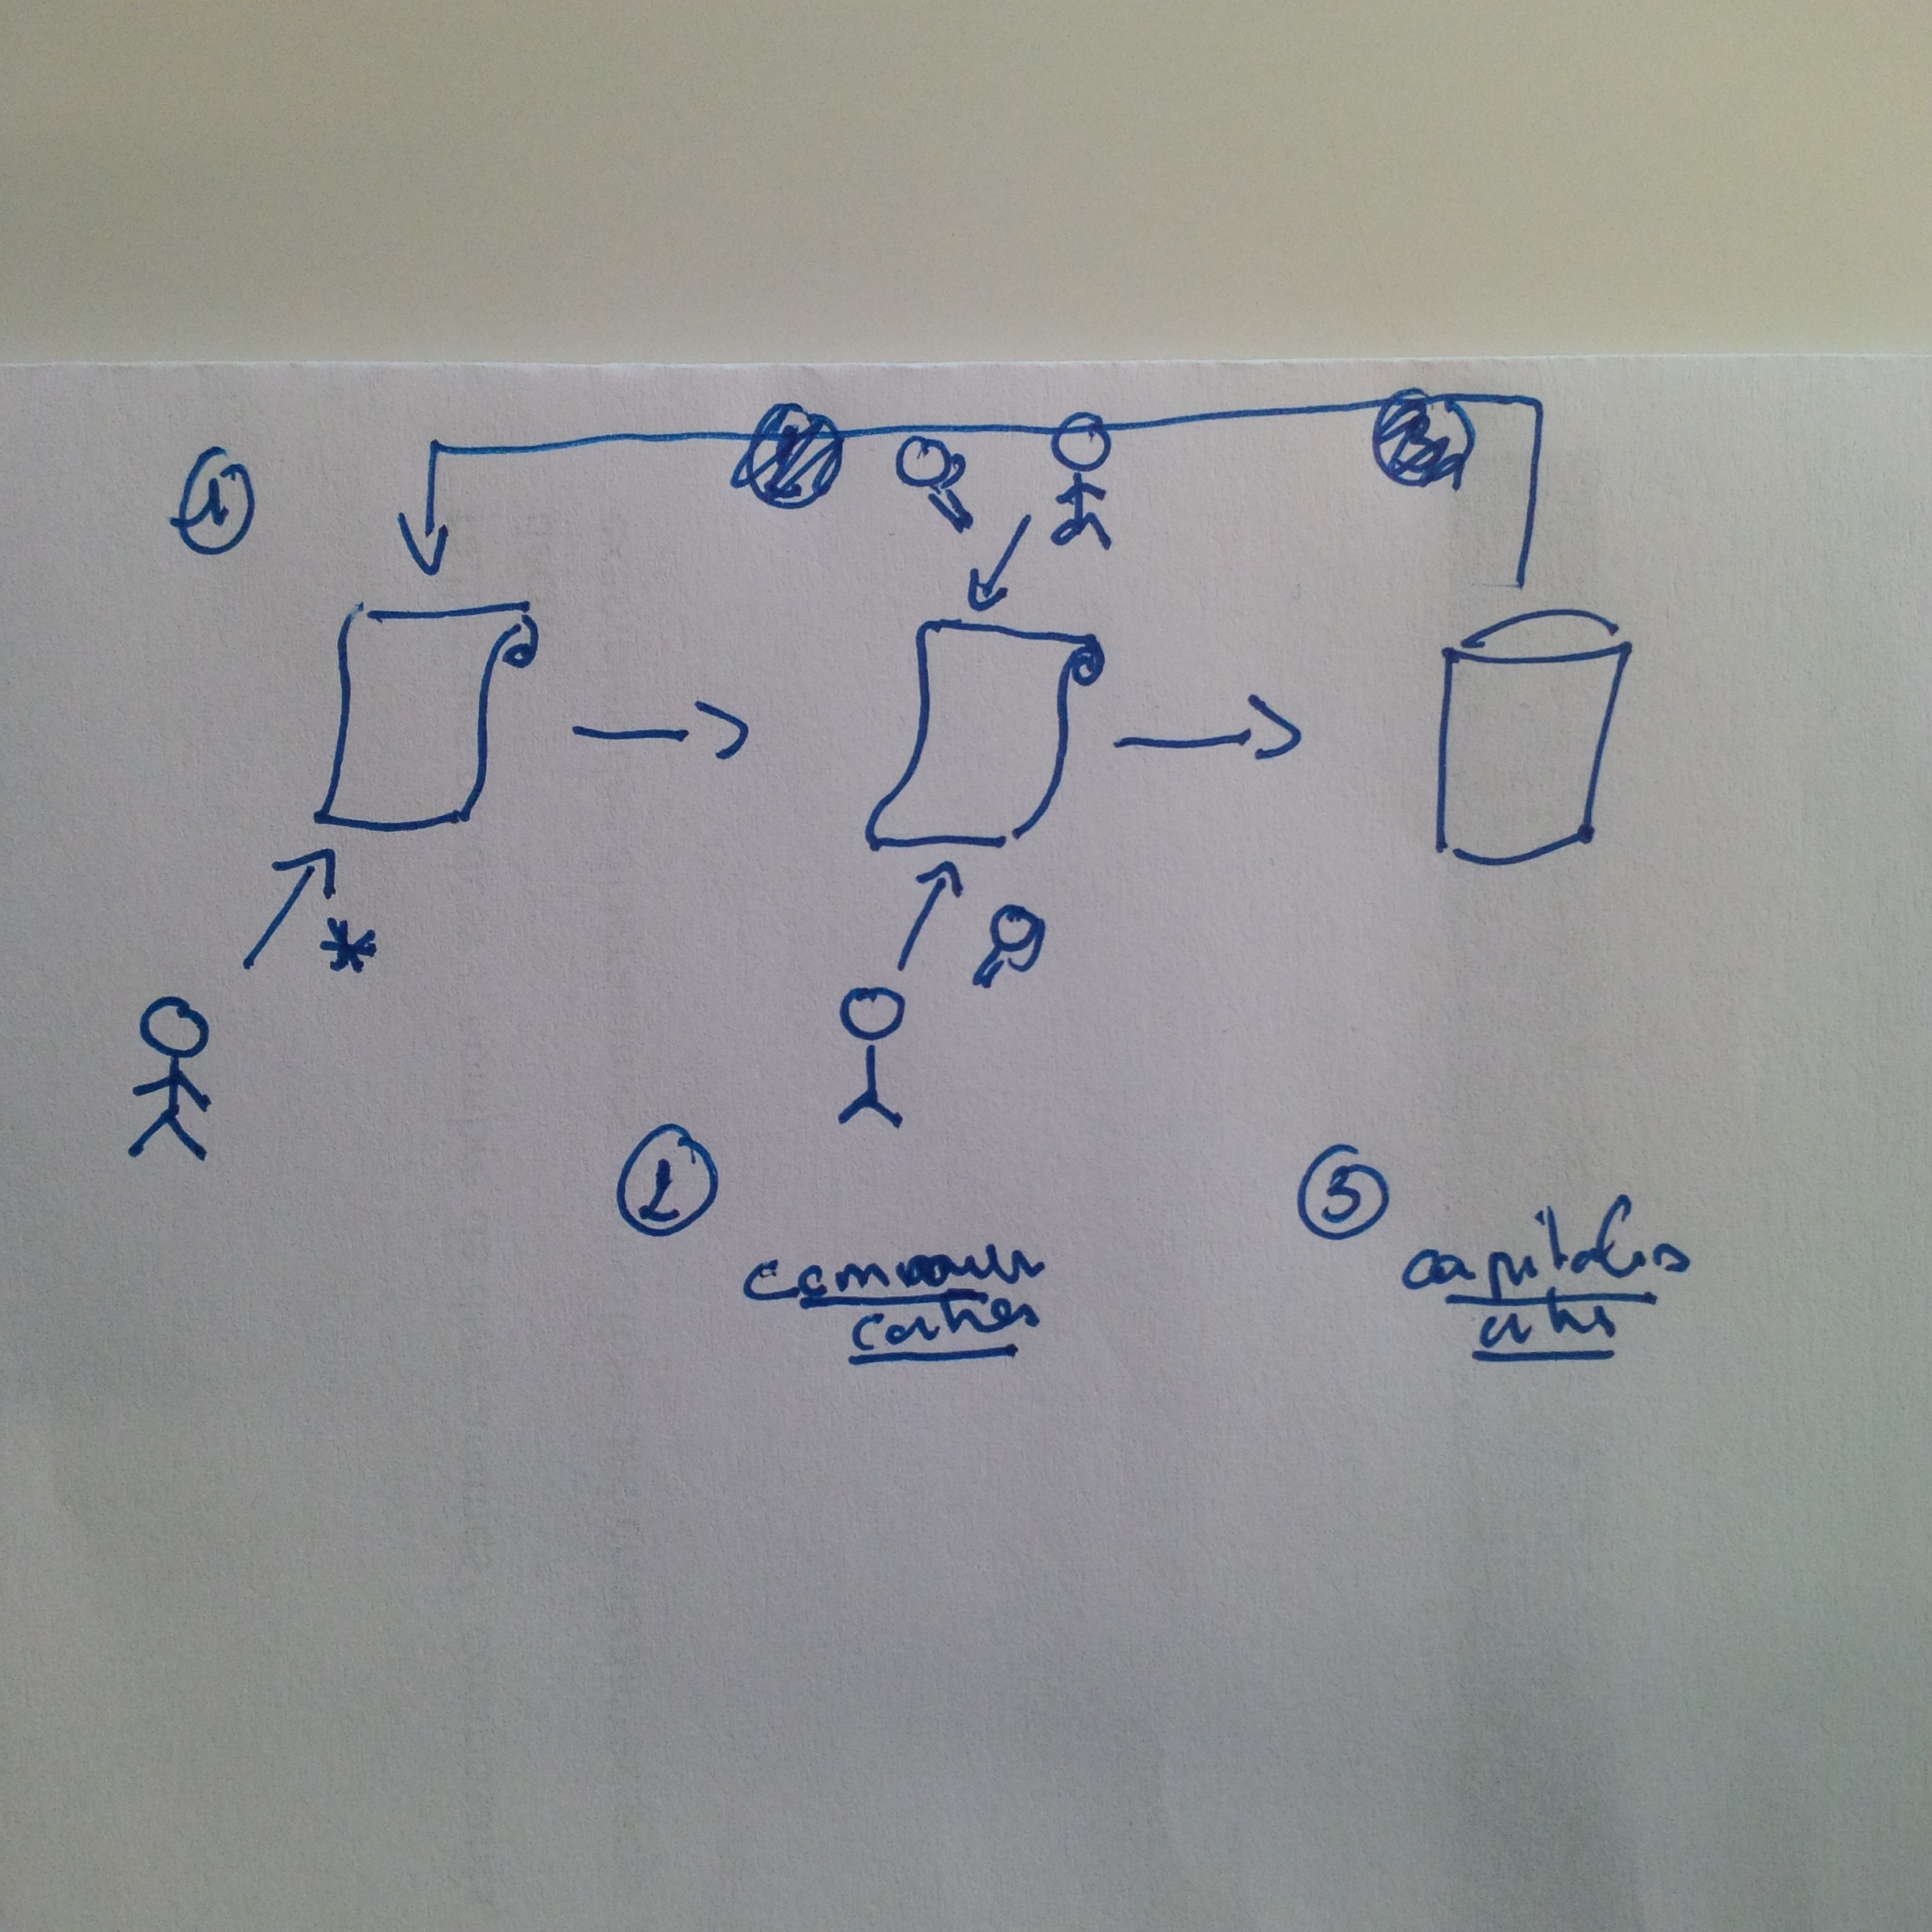
\includegraphics[width=10cm, height=3cm]{imgs/slide_application_patron}
\end{figure}
\begin{definition}
Les \textbf{patrons de conception} documentent des solutions de
conception à des problèmes de conception récurrents.
\end{definition}
\begin{exampleblock}{}
\begin{itemize}
\item Programmation orientée objet : \textit{Design Patterns: Elements of
Reusable Object-Oriented Software} 
\item Architecture des systèmes distribués : \textit{Architecture,
volume 4: A Pattern Language for Distributed Computing}
\end{itemize}
\end{exampleblock}
\end{frame}

%\begin{frame}{Problèmes rencontrés : modélisation de configuration}
%\begin{figure}
%\centering
%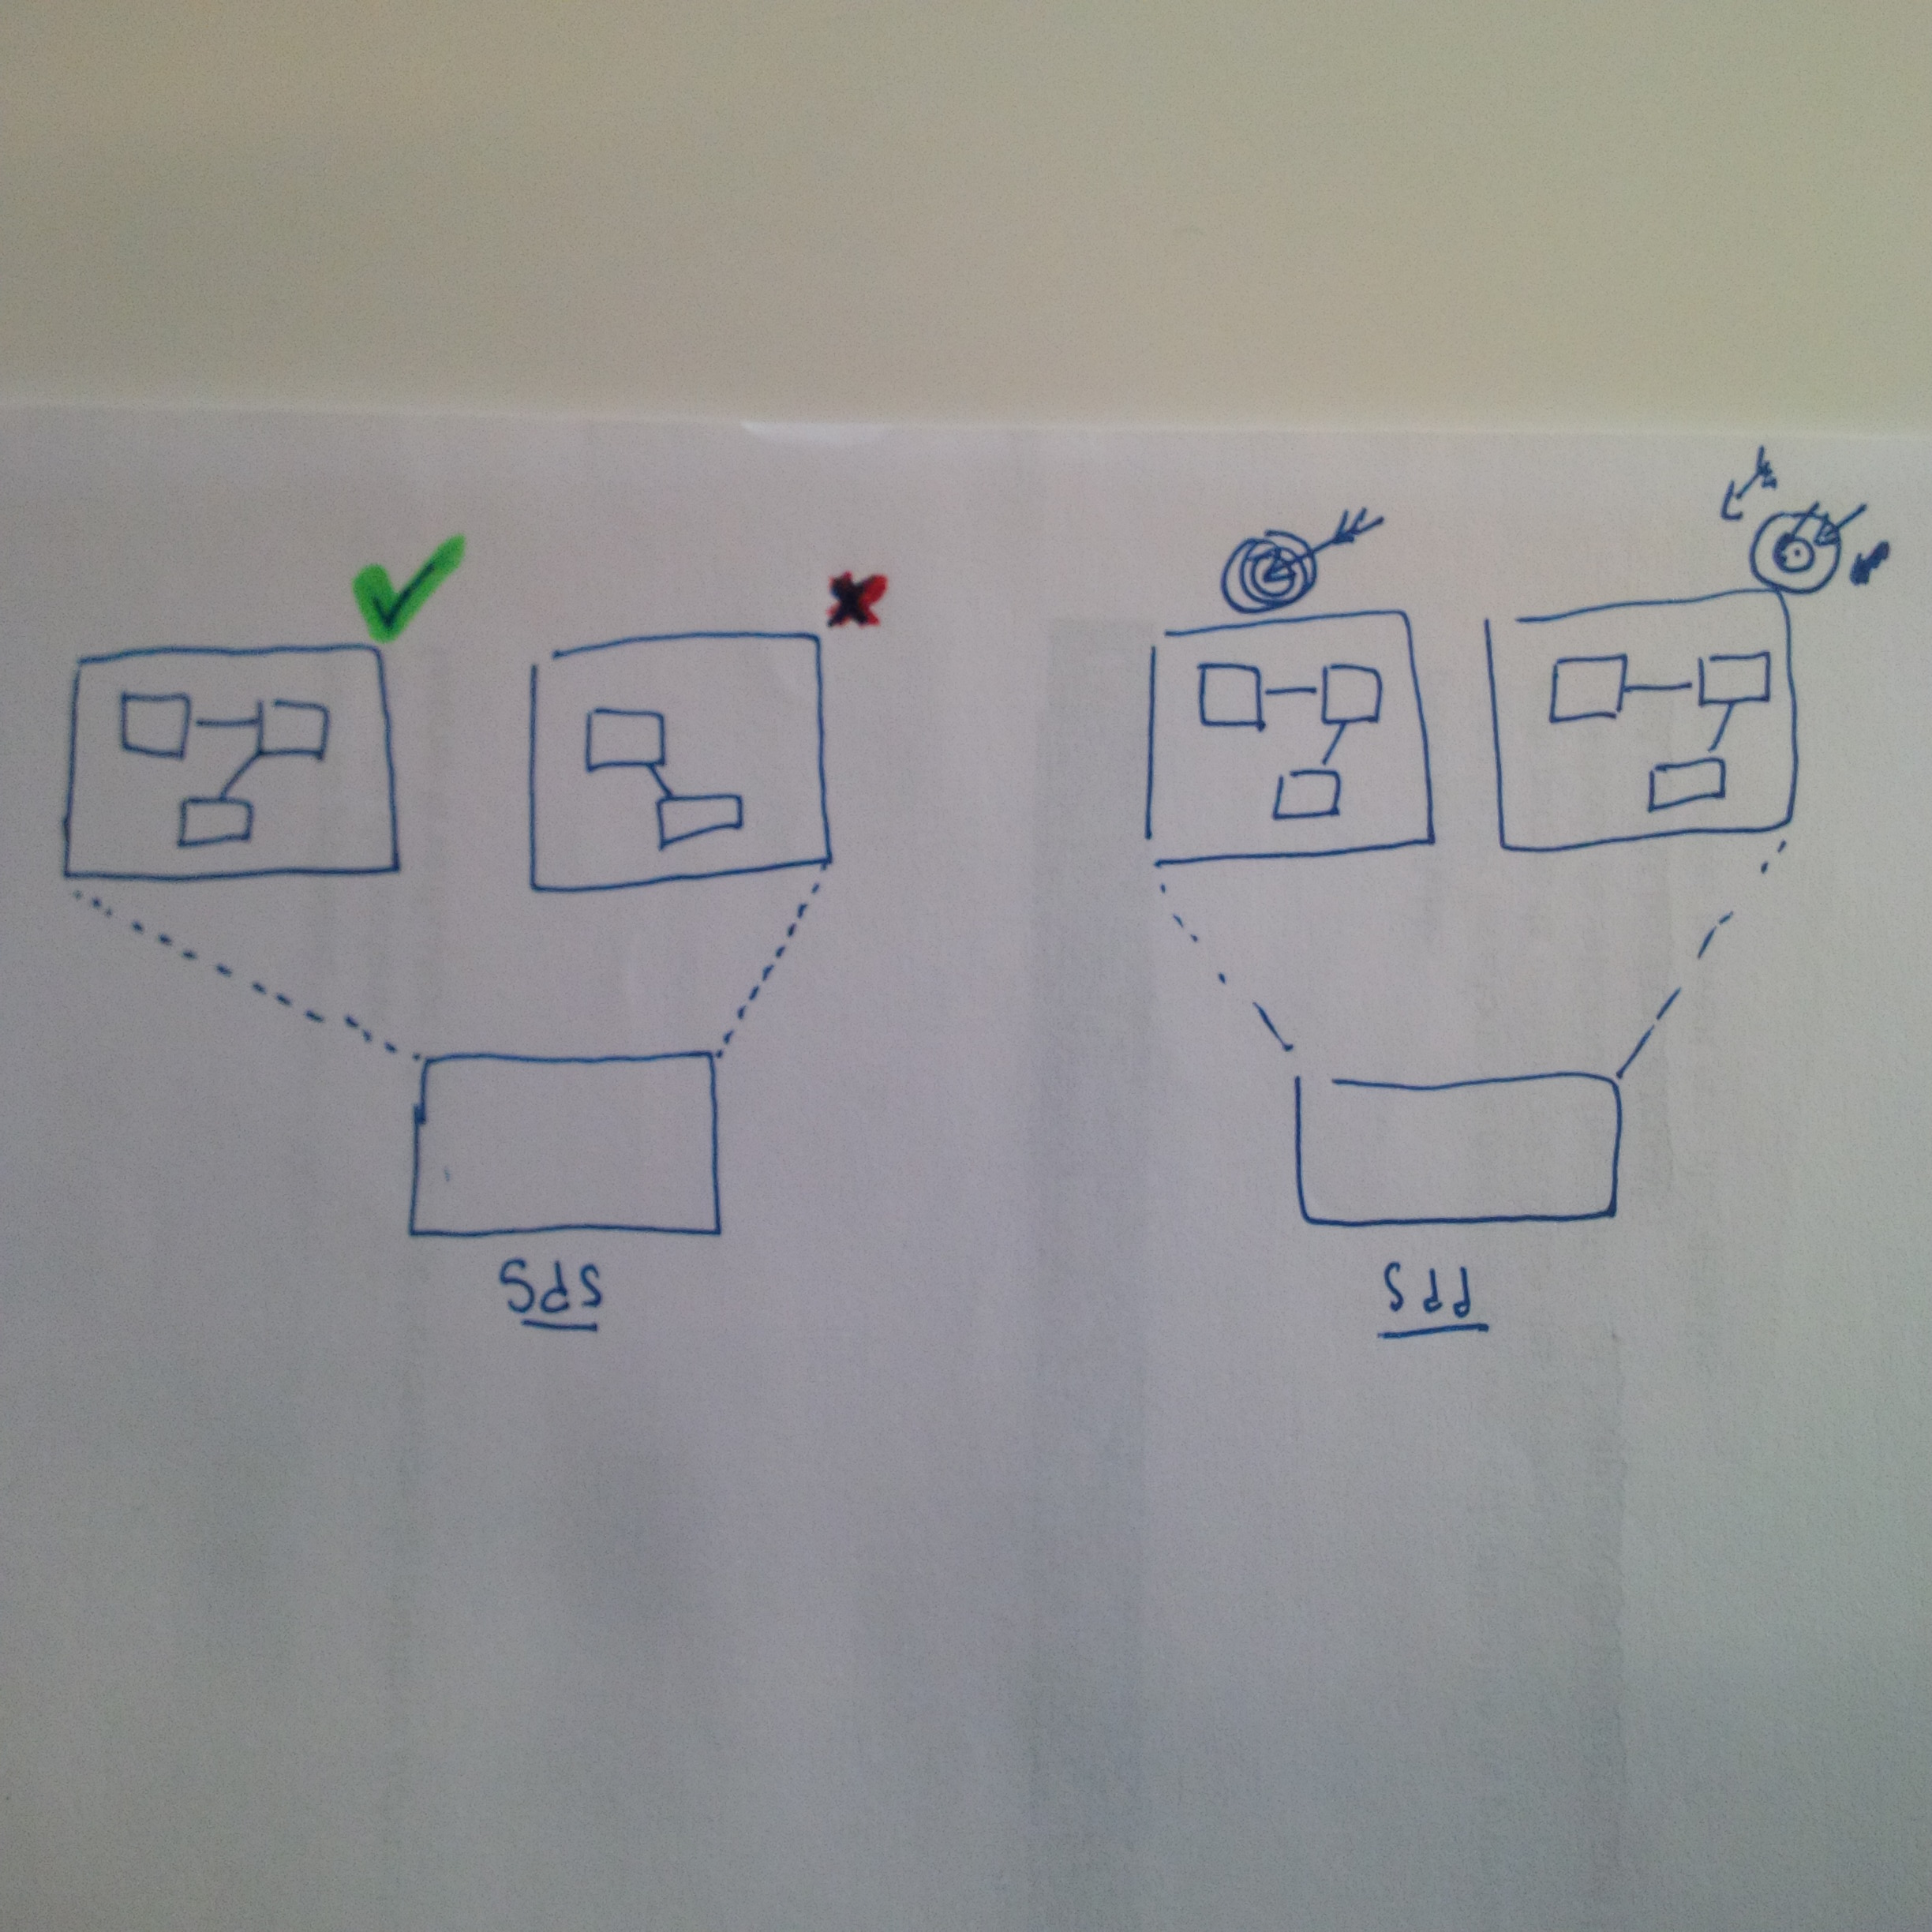
\includegraphics[width=10cm, height=4cm]{imgs/slide_probleme_modelisation.jpg}
%\end{figure} 
%\begin{definition}{}
%Un modèle est \textbf{exact} si il est
%factuel ou ne dévie pas trop du fait qu’il modélis
%\end{definition}
%\begin{definition}{}
%Un modèle est \textbf{précis} si il est suffisamment détaillé pour
%répondre au besoin de spécification, d'analyse ou de vérification.
%\end{definition}
%\end{frame}

%\begin{frame}{Problèmes recontrés : processus de reconfiguration}
%\begin{figure}
%\centering
%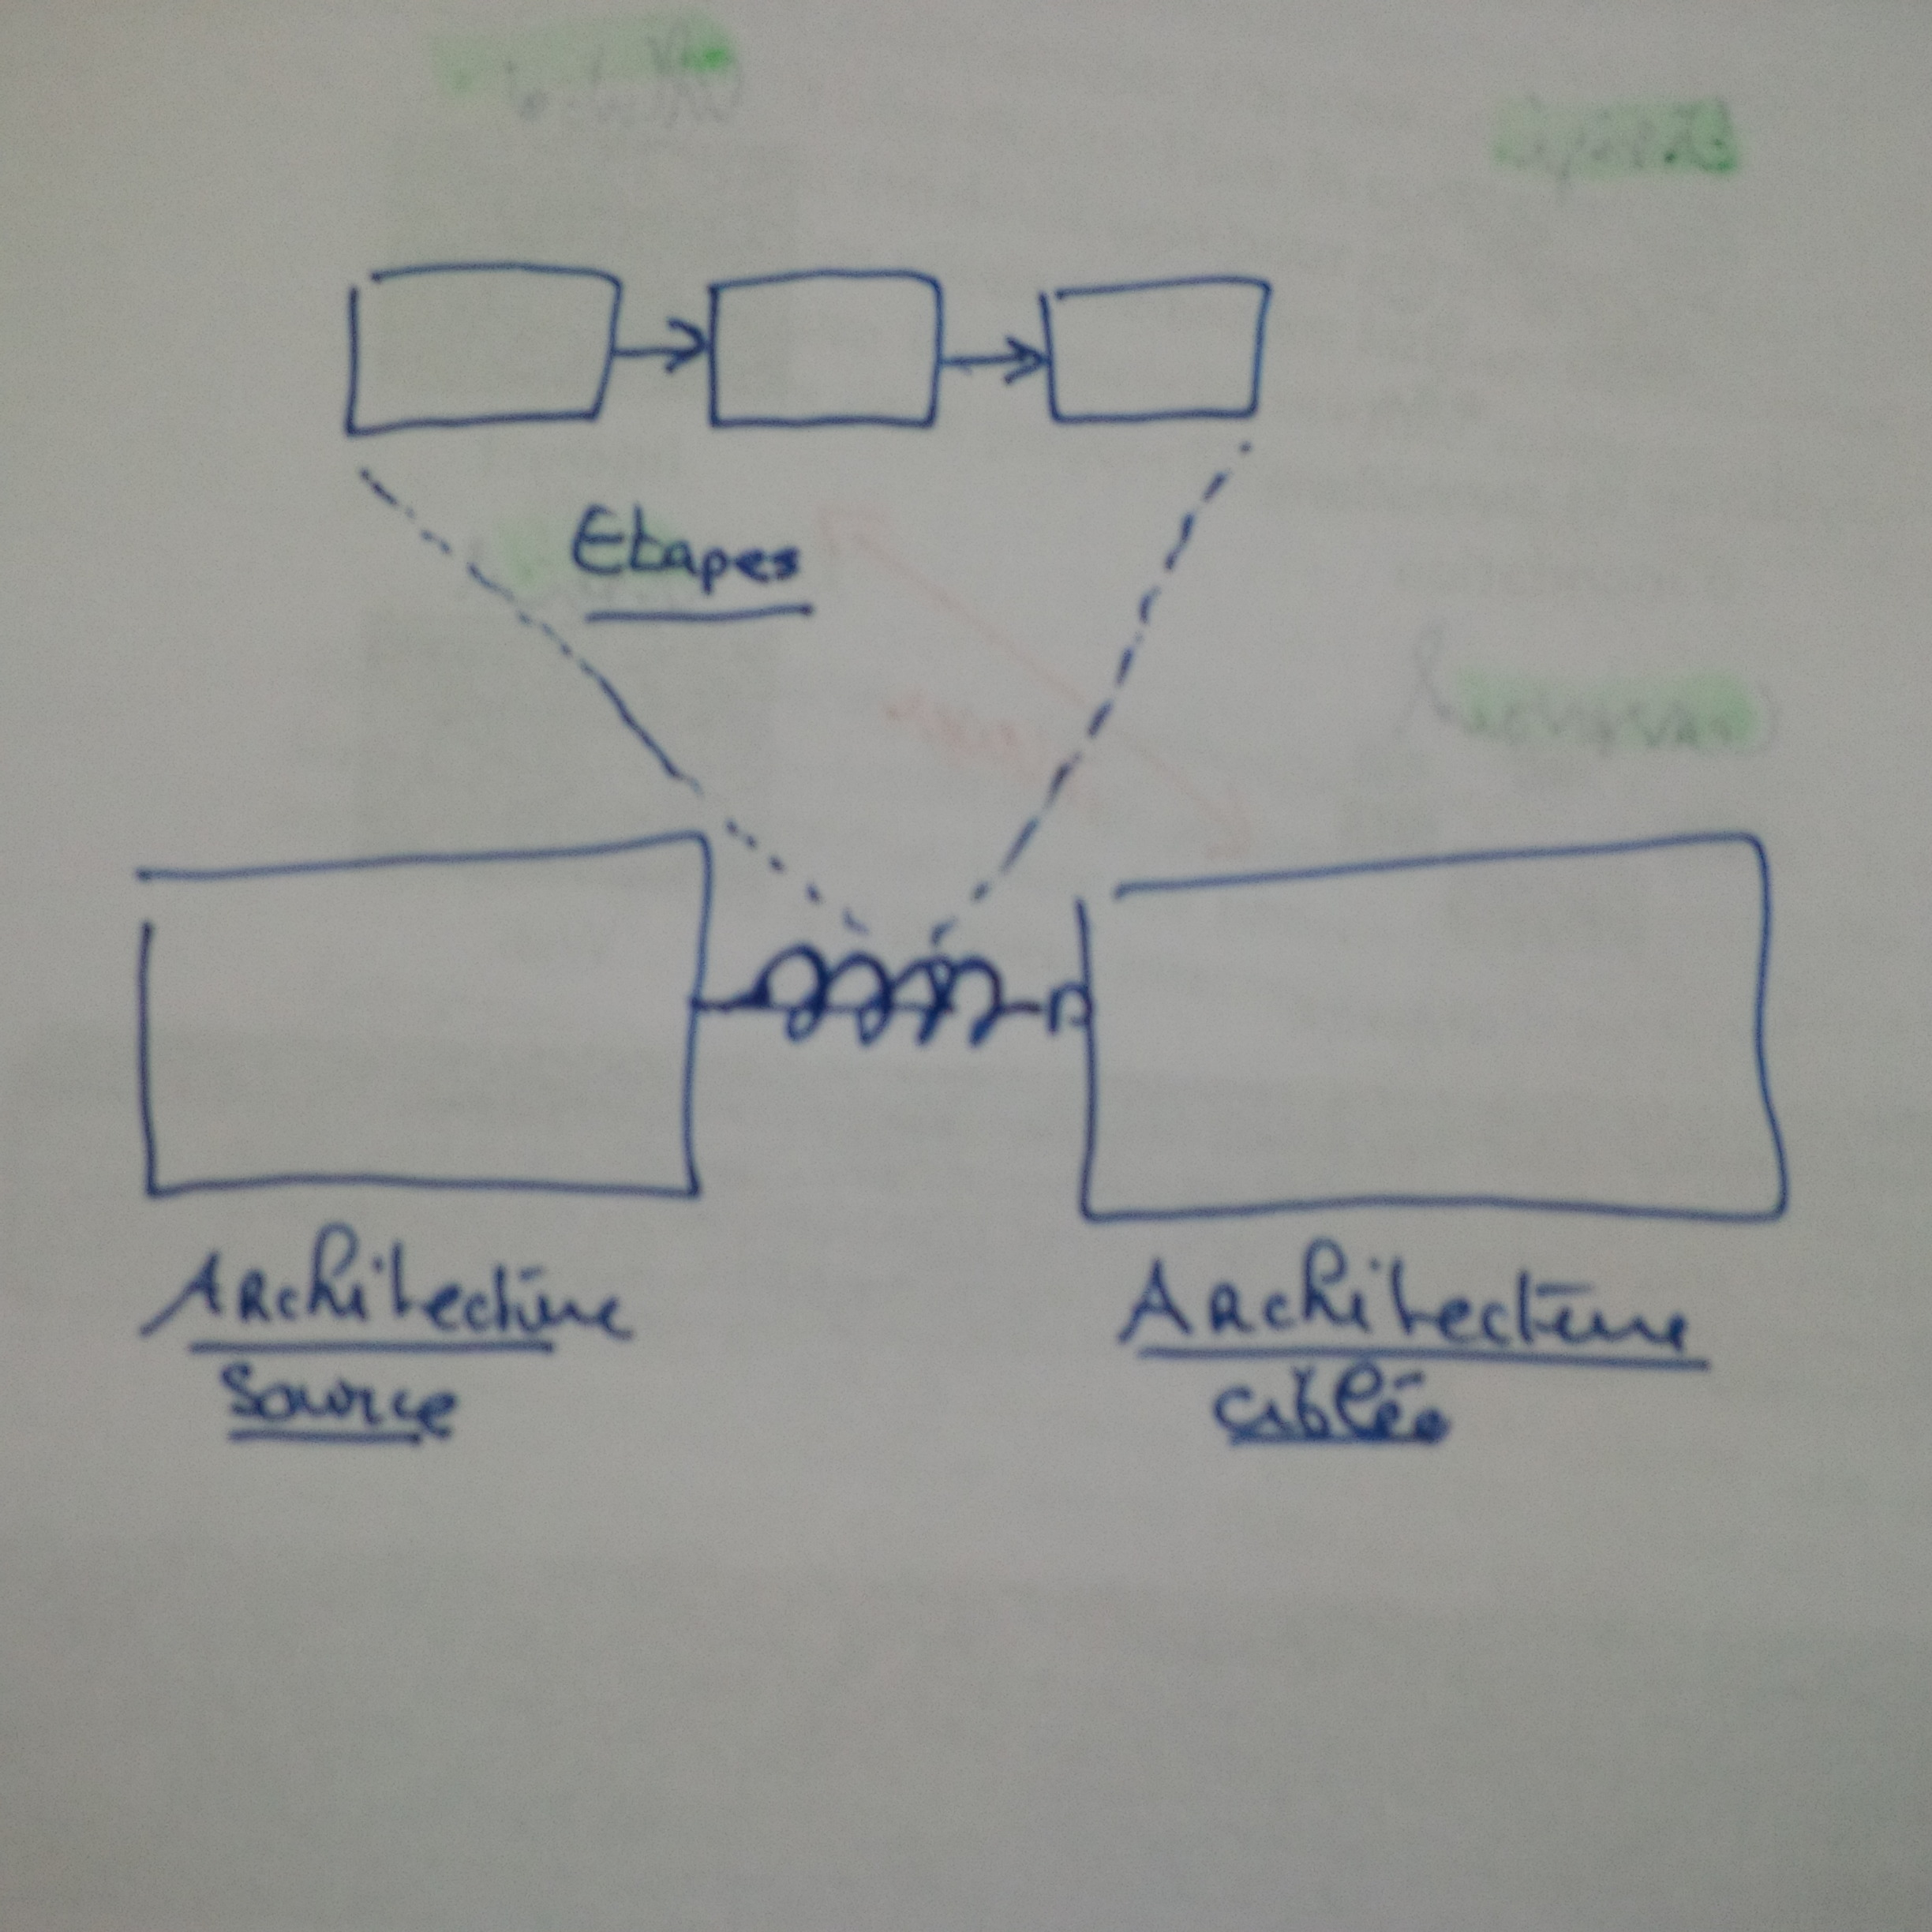
\includegraphics[width=\textwidth, height=0.6\textwidth]{imgs/slide_introduction_process.jpg}
%\end{figure}
%\end{frame}

\begin{frame}{Questions de recherche}
Comment l’architecte doit-il procéder pour faire évoluer un système de systèmes après son déploiement, dans le cadre du développement évolutionnaire ?\\
\begin{itemize}
    \item[Q1] Comment l’architecte modélise-t-il la configuration du système avec le niveau de précision et d’exactitude requis ?
    \item[Q2] Quel processus d’ingénierie l’architecte doit-il suivre pour concevoir la reconfiguration d’évolution du système de systèmes ?
    \item[Q3] Comment l’architecte peut-il documenter ses choix de conception d’une reconfiguration ?
\end{itemize}
\end{frame}

\begin{frame}{Plan de la soutenance}
\tableofcontents
\end{frame}

